\section{Introdução}

A crescente transição global para matrizes energéticas sustentáveis,
associada à eletrificação progressiva dos sistemas de transporte,
tem intensificado significativamente a demanda por tecnologias
avançadas de armazenamento de energia.
Nesse contexto, baterias baseadas em lítio consolidaram-se como
componentes centrais para a viabilização de sistemas energéticos
de alta eficiência e menor impacto ambiental. Conforme discutido por 
\textcite{machin2024advancements},o desenvolvimento de novos materiais eletroquímicos depende
fundamentalmente da compreensão microscópica das propriedades
eletrônicas que governam processos de transporte de carga,
estabilidade estrutural e reatividade química.

Porém, a descrição teórica desses fenômenos requer a determinação precisa da
estrutura eletrônica de sistemas moleculares e sólidos, tornando a
química quântica computacional uma ferramenta essencial no processo
de descoberta e otimização de materiais energéticos
\cite{kim2022fault}. Do ponto de vista fundamental, tais propriedades emergem da solução
da equação de Schrödinger independente do tempo,
\begin{equation}
\label{eq:schrodinger-eq}
\hat{H}_{mol}|\psi\rangle = E|\psi\rangle,
\end{equation}
onde $\hat{H}_{mol}$ representa o operador Hamiltoniano molecular,
responsável por descrever as contribuições cinéticas e potenciais
das partículas do sistema, $|\psi\rangle$ corresponde ao vetor de
estado eletrônico e $E$ denota a energia associada ao estado
quântico considerado.

A grande questão é que a obtenção exata das soluções de
\eqref{eq:schrodinger-eq} apresenta custo computacional que cresce
exponencialmente com o número de elétrons e orbitais envolvidos,
caracterizando o chamado problema de muitos corpos
\cite{cao2019quantum}.
Métodos clássicos de alta precisão, como o
\textit{Full Configuration Interaction} (FCI),
tornam-se rapidamente inviáveis mesmo para sistemas moleculares
moderados.
Como alternativa, abordagens aproximadas como Hartree–Fock,
Teoria do Funcional da Densidade (DFT) e métodos baseados em
\textit{Coupled Cluster} foram desenvolvidas e amplamente empregadas,
sendo estas últimas frequentemente consideradas o padrão de
referência em química computacional.
Entretanto, tais métodos apresentam limitações relevantes em regimes
de forte correlação eletrônica, frequentemente observados em
materiais de interesse tecnológico,
incluindo compostos utilizados em sistemas de armazenamento de energia
\cite{farag2022towards,tilly2022variational}.

\subsection{Formulação Eletrônica do Problema Molecular}

Sob a aproximação de Born–Oppenheimer, assume-se que os núcleos
atômicos permanecem fixos em posições definidas,
permitindo que o problema seja reduzido à dinâmica eletrônica
em um potencial nuclear estático.
Nessa formulação, o Hamiltoniano eletrônico pode ser expresso,
em segunda quantização, como
\begin{equation}
\hat{H} =
\sum_{pq} h_{pq} a_p^\dagger a_q
+
\frac{1}{2}
\sum_{pqrs} h_{pqrs}
a_p^\dagger a_q^\dagger a_r a_s,
\end{equation}
onde $a_p^\dagger$ e $a_p$ são operadores de criação e aniquilação
fermiônicos, $h_{pq}$ representam integrais de um elétron
e $h_{pqrs}$ descrevem as interações eletrônicas de dois corpos.

O número de termos associados às interações de dois elétrons cresce
rapidamente com o número de orbitais considerados,
aumentando significativamente a complexidade computacional.
Para tornar o problema tratável, técnicas de redução dimensional,
como métodos de espaço ativo,
são frequentemente empregadas.
Além disso, decomposições de baixo posto,
como a decomposição de Cholesky,
permitem fatorar o tensor de interações eletrônicas em formas
mais compactas e computacionalmente eficientes
\cite{cohn2021quantum, motta2018lowrank}.

Após essa etapa, o Hamiltoniano fermiônico pode ser mapeado
para operadores de spin por meio de transformações
fermion–qubit, como a transformação de Jordan–Wigner,
viabilizando sua implementação em dispositivos quânticos digitais.

\subsection{Computação Quântica e Representação de Sistemas Físicos}

A computação quântica emerge, portanto, como alternativa natural
para a simulação de sistemas quânticos complexos,
explorando diretamente os princípios físicos que governam tais sistemas.
A proposta original, formulada por \textcite{feynman1982simulating},
baseia-se na observação de que sistemas quânticos são descritos
de forma mais eficiente por dispositivos igualmente quânticos.

Diferentemente da computação clássica, na qual a informação é codificada
em bits binários pertencentes ao conjunto $\{0,1\}$,
a informação quântica é representada por vetores normalizados em
espaços vetoriais complexos de dimensão finita, usualmente descritos
em termos de qubits \textcite{nielsen2000quantum}.

Um qubit pode ser escrito como uma superposição linear dos estados
computacionais base $|0\rangle$ e $|1\rangle$,
\begin{equation}
|\psi\rangle = \alpha |0\rangle + \beta |1\rangle,
\end{equation}
onde $\alpha, \beta$ são complexos e satisfazem
$|\alpha|^2 + |\beta|^2 = 1$.

A representação geométrica de um único qubit pode ser visualizada
na esfera de Bloch (Figura~\ref{fig:bloch}).
Observa-se que o vetor de estado não está alinhado exclusivamente com os 
polos $|0\rangle$ ou $|1\rangle$, mas ocupa uma posição intermediária na 
superfície da esfera, assim, caracterizando uma superposição coerente. A 
posição angular do vetor na esfera é parametrizada pelos ângulos $\theta$ e 
$\phi$, os quais determinam, respectivamente, as amplitudes relativas e a 
fase global do estado quântico. \begin{figure}[htb] \centering 
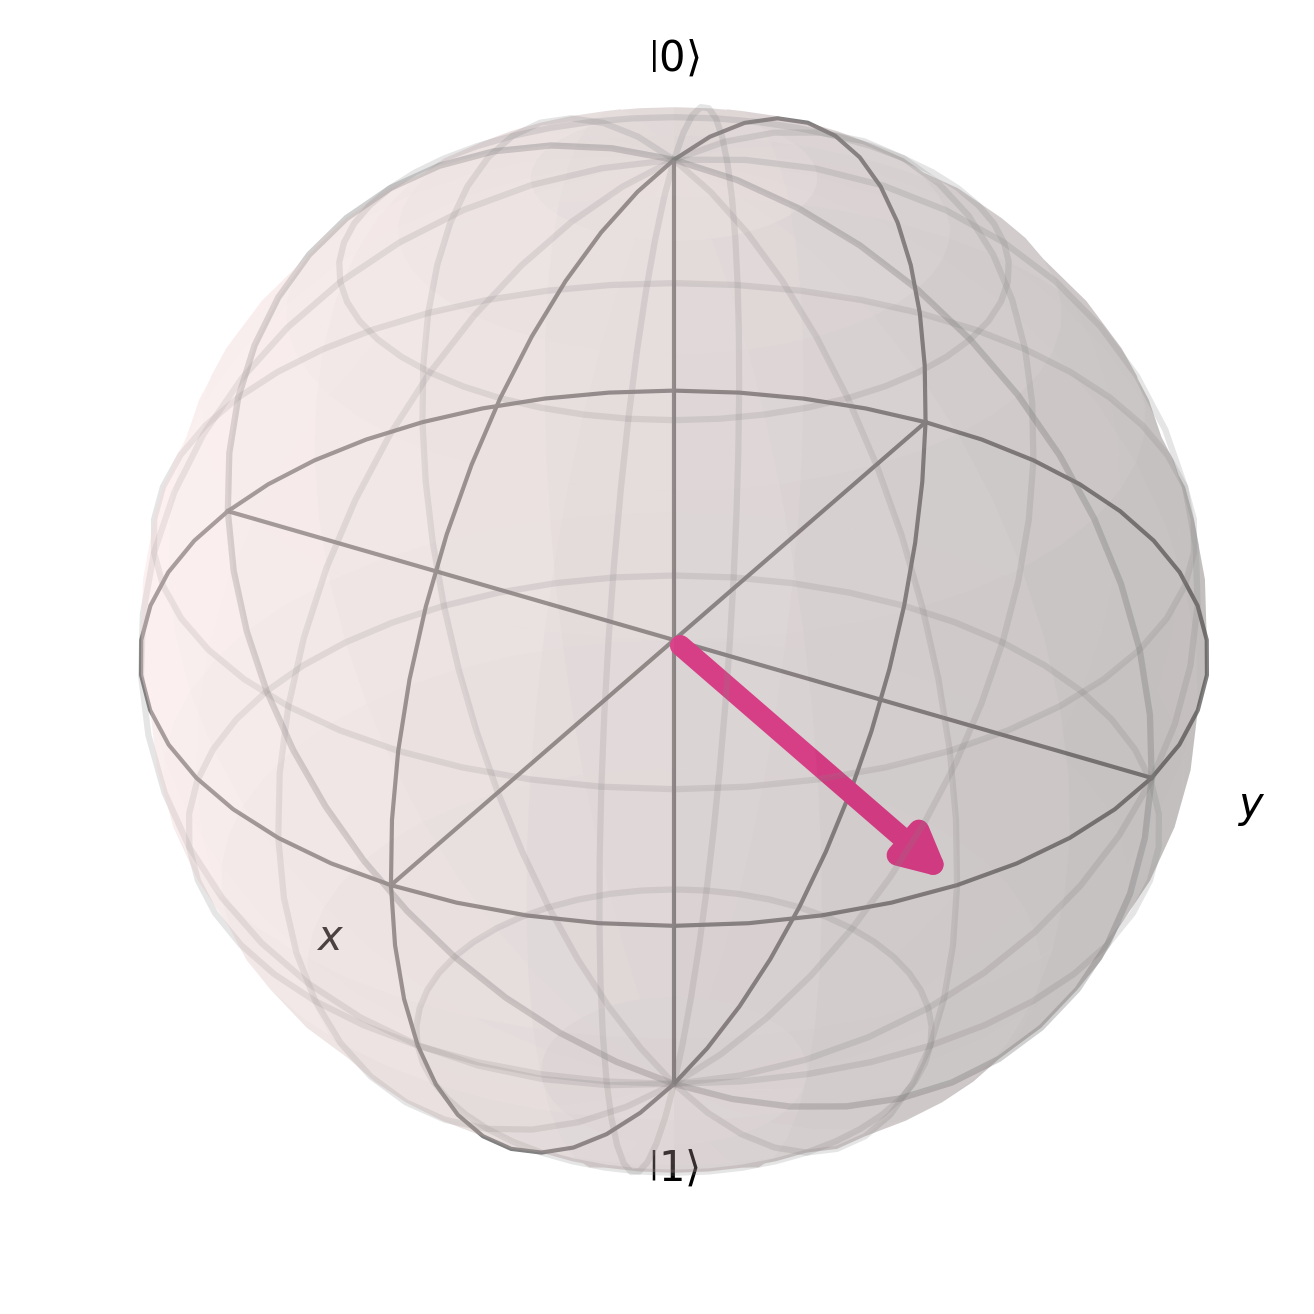
\includegraphics[width=0.4\textwidth]{img/bloch_sphere.png} 
\caption{Representação geométrica de um qubit em superposição na esfera de 
Bloch. Fonte: elaboração própria com Qiskit (2026).} \label{fig:bloch} 
\end{figure}

A evolução temporal de estados quânticos é descrita por operadores
unitários, isto é, transformações lineares que preservam a norma
do vetor de estado no espaço de Hilbert.
No contexto computacional, tais operadores são implementados
fisicamente na forma de portas quânticas, análogas às portas
lógicas da computação clássica, porém descritas por matrizes
unitárias.

Como exemplo fundamental, destaca-se a porta Controlled-NOT (CNOT),
responsável por introduzir correlações entre dois qubits.
Em representação matricial, considerando a base computacional
$\{|00\rangle, |01\rangle, |10\rangle, |11\rangle\}$,
a CNOT é dada por
\begin{equation}
\text{CNOT} =
\begin{pmatrix}
1 & 0 & 0 & 0 \\
0 & 1 & 0 & 0 \\
0 & 0 & 0 & 1 \\
0 & 0 & 1 & 0
\end{pmatrix}.
\end{equation}
essa operação preserva o qubit de controle e inverte o qubit alvo
quando o controle se encontra no estado $|1\rangle$,
sendo um dos elementos essenciais para a geração de emaranhamento.

\subsection{Circuitos Quânticos e Estados Parametrizados}

No modelo computacional baseado em portas quânticas,
operações físicas são implementadas por sequências de operadores
unitários organizados em circuitos quânticos.
Cada circuito define uma transformação no espaço de estados,
permitindo a preparação controlada de estados quânticos
complexos a partir de estados iniciais simples.

A Figura~\ref{fig:quantum_circuit} apresenta um exemplo
esquemático de circuito quântico parametrizado.
Observa-se que as rotações $R_y(\theta)$ e $R_z(\phi)$
introduzem graus de liberdade contínuos no espaço de estados,
enquanto a porta CNOT, previamente definida, promove correlações
quânticas entre os qubits por meio de uma transformação unitária
não separável, o emaranhamento.

\begin{figure}[H]
\centering
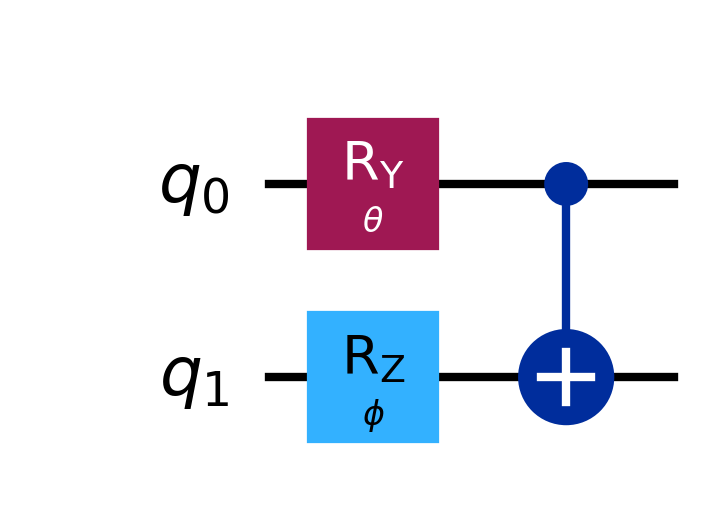
\includegraphics[width=0.4\textwidth]{img/parametrized_circuit.png}
\caption{Exemplo de circuito quântico parametrizado utilizado na preparação de estados variacionais. Fonte: elaboração própria com Qiskit (2026).}
\label{fig:quantum_circuit}
\end{figure}

Circuitos contendo parâmetros ajustáveis constituem a base dos
chamados \textit{ansätze variacionais},
nos quais rotações quânticas dependentes de parâmetros clássicos
definem famílias contínuas de estados candidatos.
Ou seja, ao variar continuamente esses parâmetros, o circuito pode preparar
uma infinidade de vetores distintos no espaço de Hilbert,
explorando diferentes configurações eletrônicas possíveis.
Essa característica torna possível adaptar o estado quântico
preparado de modo a aproximar soluções físicas de interesse,
como estados fundamentais moleculares.

\subsection{A Era NISQ e Algoritmos Variacionais}
\label{sec:nisq_variational}

Apesar do avanço experimental significativo,
os dispositivos quânticos atualmente disponíveis ainda operam sob
fortes limitações de coerência (tempo durante o qual a informação quântica é preservada),
fidelidade de portas (precisão na execução das operações quânticas)
e número de qubits disponíveis.
Esses sistemas são classificados como dispositivos
\textit{Noisy Intermediate-Scale Quantum} (NISQ),
terminologia introduzida por Preskill
\cite{preskill2018nisq}.
O termo descreve a geração atual de computadores quânticos,
que possuem dezenas ou poucas centenas de qubits,
mas ainda não contam com correção completa de erros.
Nesse regime, algoritmos quânticos tradicionais, como aqueles baseados
em circuitos profundos e longas sequências de portas,
tornam-se impraticáveis devido ao acúmulo de ruído e à rápida perda de coerência.
Consequentemente, o desenvolvimento de algoritmos especificamente
adaptados às restrições experimentais atuais tornou-se uma das principais
linhas de pesquisa em computação quântica aplicada
\cite{bharti2021noisy}.

A determinação do estado fundamental de um sistema físico pode ser
formulada como um problema de autovalores associado ao Hamiltoniano
molecular, isto é, à representação matemática da energia total do sistema.
O princípio variacional da mecânica quântica estabelece que o valor
esperado da energia calculado para qualquer estado normalizado
constitui um limite superior para a energia do estado fundamental,
\begin{equation}
E(\theta)=\langle \psi(\theta)|\hat{H}|\psi(\theta)\rangle.
\end{equation}
em termos físicos, isso significa que,
ao testar diferentes estados candidatos,
nunca se obtém um valor inferior à energia real do estado fundamental.
Essa propriedade permite transformar o problema quântico original,
encontrar o menor autovalor de um operador,
em um problema de otimização,
no qual se busca minimizar a energia esperada.

Ao conectar a formulação eletrônica do problema molecular
à capacidade de manipulação de estados quânticos por meio de
circuitos parametrizados,
os algoritmos variacionais emergem como solução natural
no contexto da era NISQ, conforme afirma \textcite{hidary2019quantum}.
Entre esses algoritmos, destaca-se o
\textit{Variational Quantum Eigensolver} (VQE),
introduzido por Peruzzo et al.~\cite{peruzzo2014variational},
que combina preparação de estados quânticos parametrizados
com otimização clássica iterativa,
permitindo estimar energias fundamentais moleculares
mesmo sob restrições experimentais atuais.
Ou seja, essa arquitetura combina:
a capacidade dos dispositivos quânticos de preparar estados
altamente entrelaçados, difíceis de simular classicamente, juntamente
com a eficiência de algoritmos clássicos na otimização numérica.

Dessa forma, um circuito quântico parametrizado prepara estados
candidatos dependentes de parâmetros variacionais $\theta$.
Em seguida, as medições realizadas no hardware quântico
fornecem estimativas da energia esperada.
Um otimizador clássico então atualiza iterativamente os parâmetros
com o objetivo de minimizar essa energia.

O ciclo operacional do VQE encontra-se ilustrado na
Figura~\ref{fig:vqe_cycle}. 
O processo consiste essencialmente em:
(i) preparação do estado parametrizado,
(ii) medição de observáveis,
(iii) avaliação da função custo e
(iv) atualização clássica dos parâmetros,
sendo o ciclo repetido até convergência energética, logo, até que a 
variação energética entre iterações torne-se suficientemente pequena.
\cite{mcclean2016theory}.

\begin{figure}[H]
\centering
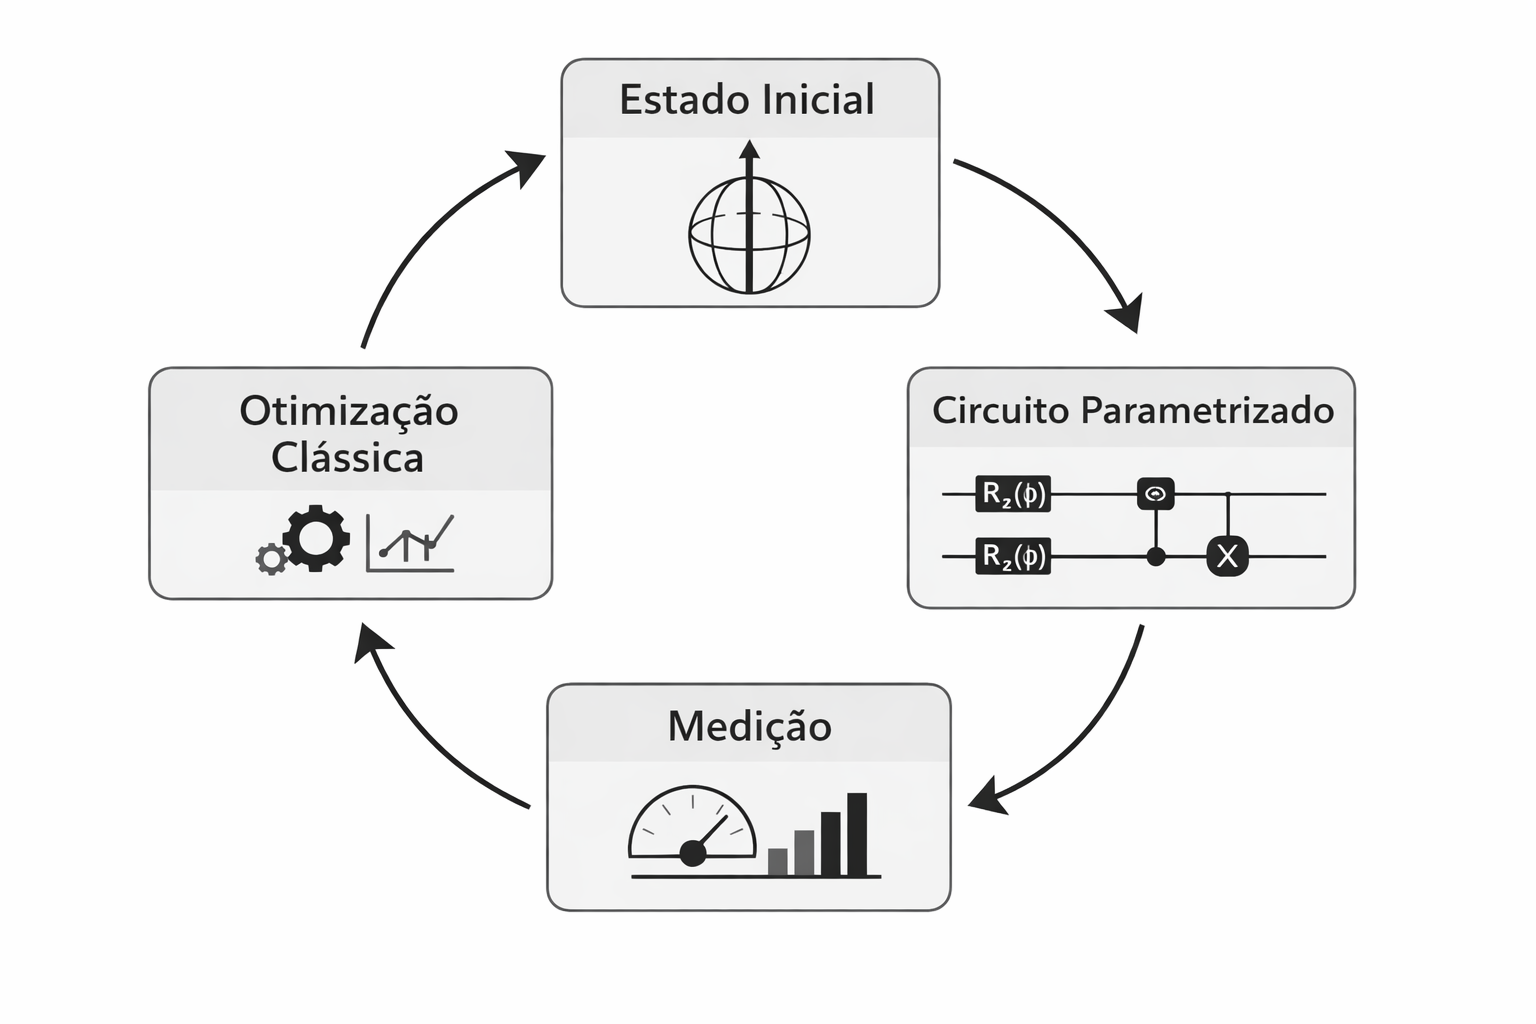
\includegraphics[width=0.5\textwidth]{img/vqe_cycle.png}
\caption{Fluxo híbrido do algoritmo VQE envolvendo etapas quânticas e 
clássicas. Fonte: elaboração própria (2026).}
\label{fig:vqe_cycle}
\end{figure}

Devido à possibilidade de utilização de circuitos relativamente rasos,
isto é, com menor profundidade e, portanto, menor acúmulo de ruído
e à sua natureza híbrida, o VQE consolidou-se como uma das estratégias
mais promissoras para simulação molecular em dispositivos quânticos
atuais \cite{tilly2022variational}.
Diante desse cenário, torna-se relevante investigar de forma sistemática
a implementação prática de algoritmos variacionais voltados à simulação
de sistemas moleculares.

Por fim, o presente trabalho concentra-se na consolidação conceitual,
reimplementação e validação do algoritmo VQE utilizando o
ecossistema Qiskit como ambiente principal de desenvolvimento.
Embora a etapa atual deste projeto concentre-se em sistemas 
moleculares modelo,
como H$_2$ e LiH, essa abordagem estabelece as bases conceituais
e computacionais necessárias para extensões futuras envolvendo
materiais mais complexos relevantes para tecnologias de
armazenamento de energia, bem como a integração de técnicas
de aprendizado de máquina para análise e otimização das
simulações quânticas realizadas.
